\documentclass{ctexart}
\usepackage[left=1.5cm,right=1.5cm,top=1.5cm,bottom=1.5cm]{geometry}
\usepackage{listings}
\usepackage[dvipsnames]{xcolor}
\usepackage{cite}
\usepackage{diagbox}
\usepackage{fancyhdr} % 加载fancyhdr宏包,用于设置页眉和页脚
\pagestyle{fancy} % 设置页面样式
\fancyhf{} % 清除默认的页眉和页脚的内容
\fancyfoot[C]{\thepage} 
\renewcommand{\headrulewidth}{0pt} % 将页眉的横线宽度设置为0pt

\usepackage{graphicx}
\usepackage{longtable}
\usepackage{tabularx}
\usepackage{float}
\usepackage{amsmath}%引用宏包要放在documentclass后面,否则报错
\usepackage{hyperref}
\usepackage{bm}
\usepackage{amssymb}
\usepackage{esint}
\usepackage{booktabs}
%\usepackage{subfiles}%用于分章节管理引用,使各章节引用来源于各自的文件,编号相互独立
\usepackage{amsthm}
\title{数字电路实验\quad 实验报告5}
\author{Leo}
\date{\today}

\begin{document}
\maketitle
\section{实验内容}
用两个D触发器设计一个流水灯,流水灯有四个LED灯组成。具体要求为
\begin{enumerate}
    \item 使用D触发器芯片
    \item 列出状态转移真值表和转换图
    \item 给出电路实现方案
    \item 调试电路,实现始终三亮一暗,右移
\end{enumerate}
\section{实验器材}
Pocketlab、电脑、导线若干、剥线钳、镊子、限流电阻4个、红色LED灯4个、7400芯片一个、7474芯片一个部分芯片的引脚图如下所示
\begin{figure}[H]
    \centering
    \begin{minipage}{0.5\textwidth}
    \centering
           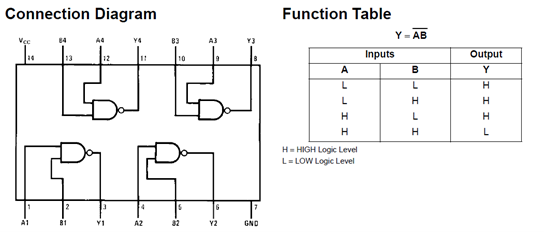
\includegraphics[width=0.8\textwidth]{7400.png}
           \caption{7400}
    \label{}
    \end{minipage}
    \hspace{0.05\textwidth}
    \begin{minipage}{0.3\textwidth}
    \centering
           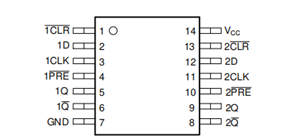
\includegraphics[width=0.8\textwidth]{7474.png}
           \caption{7474}
    \label{7474}
    \end{minipage}
\end{figure}
\section{实验原理}
题目要求实现四个流水灯交替点亮和熄灭,这意味着有4种状态需要编码,而一个触发器有两种状态,所以使用两个触发器正好可以实现。(其实若将时钟信号也用于编码,则只需要一个触发器即可实现,但是这既不常见也不符合题目要求,故不采取这种编码方式)

首先来介绍一下图\ref*{7474}所示的7474芯片。这是2路D类上升沿触发器,除了电源引脚Vcc和接地引脚GND,还有一些引脚需要注意:
\begin{enumerate}
    \item $\overline{PRE}:$异步置1端。只要输入为有效电平(低电平),则输出$Q=H,\overline{Q}=L$
    \item $\overline{CLR}:$异步清零端。只要输入为有效电平(低电平),则输出$Q=L,\overline{Q}=H$
    \item $\overline{CLK}:$时钟端。注意两个触发器的时钟是不共用的
\end{enumerate}
值得注意的是,当异步置1端和异步清零端同时为有效电平时,$Q=\overline{Q}=H$,但是这种情况是不稳定的,一旦有一个端子不再为有效电平,就会出现不确定情况,因此需要避免异步置1端和异步清零端同时为有效电平。下面是完整的功能表
\begin{figure}[H]
    \centering
    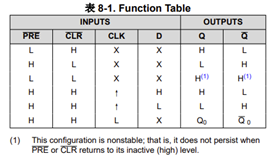
\includegraphics[width=0.6\textwidth]{7474真值表.png}
    \caption{7474完整功能表}
\end{figure}
我们由时序电路分析的经验可以知道,如果将D触发器的$\overline{Q}$接到自身的时钟端,则可以实现分频器的功能,即将脉冲的频率变为原先的一半。若将两个D触发器级联,把上一个触发器的输出$Q$作为下一级触发器的时钟,并将下一级再次分频,则还可以再把频率降为上一级的一半。这样就会出现四种状态编码,满足设计需求。在Multisim中做出电路图
\begin{figure}[H]
    \centering
    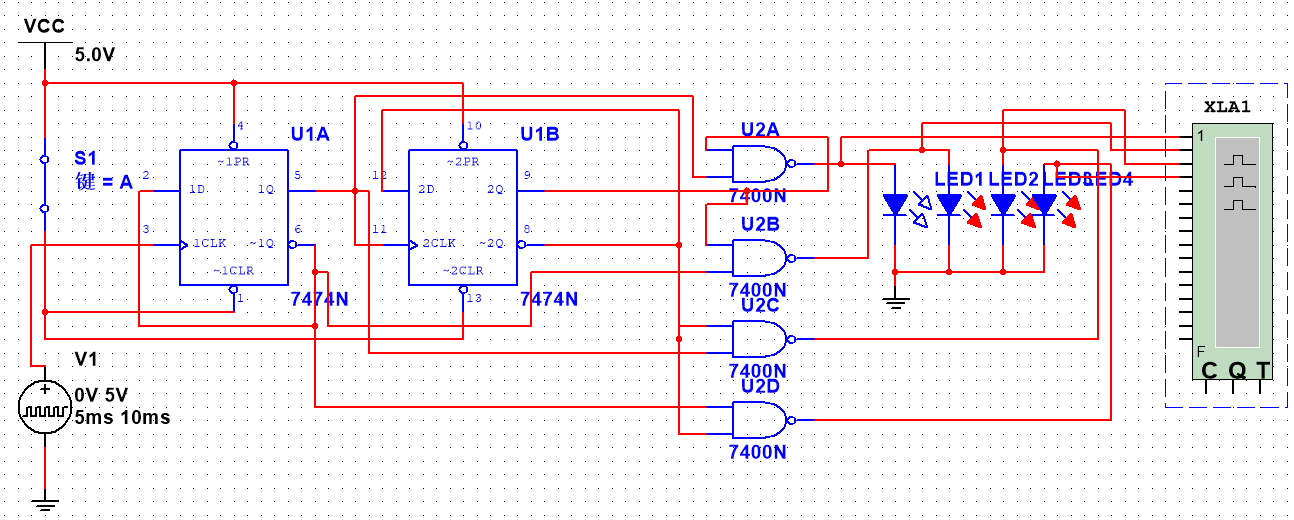
\includegraphics[width=0.6\textwidth]{multisim.png}
    \caption{multisim}
    \label{multisim}
\end{figure}
理论上时序图应该如下图所示
\begin{figure}[H]
    \centering
    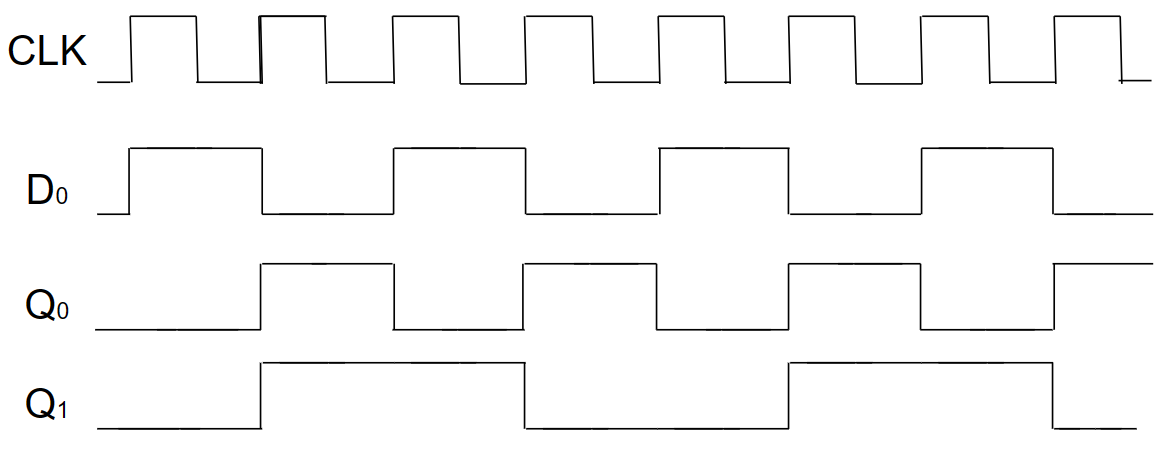
\includegraphics[width=0.6\textwidth]{时序图.png}
    \caption{时序图}
\end{figure}
利用$Q_1Q_0$编码。因为对于单个灯来说,在四个编码里只有一个情况不亮,很容易想到用最小项的非来表示。不妨定义四个灯为$L_0-L_4$,定义它们的编码:
\begin{align}
    L_3=(Q_2Q_1)'\\
    L_2=(Q_2Q_1')'\\
    L_1=(Q_2'Q_1)'\\
    L_0=(Q_2'Q_1')'\\
\end{align}
写出驱动方程即可得到状态转移方程
\begin{align}
    Q_0^{n+1}=D_0=\overline{Q_0^n}[CP\uparrow]\\
    Q_1^{n+1}=D_1=\overline{Q_1^n}[Q_{0}\uparrow]\\
\end{align}
列出状态转移真值表
\begin{table}[H]
    \centering
    \caption{状态转移真值表}
    \begin{tabular}{cccccc}
    \hline 
        $Q_1^n$ & $Q_0^n$ & $Q_1^{n+1}$ & $Q_1^{n+1}$ & CP & $Q_0$\\ \hline 
        0 & 0 & 1 & 1 & $\uparrow$ & $\uparrow$\\
        1 & 1 & 1 & 0& $\uparrow$ & -\\
        1 & 0 & 0 & 1& $\uparrow$ & $\uparrow$\\
        0 & 1 & 0 & 0& $\uparrow$ & -\\ \hline 
    \end{tabular}
    \label{状态转移真值表}
\end{table}
根据状态转移真值表可以画出状态转换图
\begin{figure}[H]
    \centering
    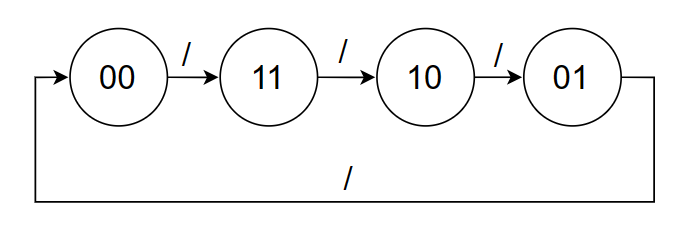
\includegraphics[width=0.6\textwidth]{状态转换图.png}
    \caption{状态转换图}
\end{figure}
\section{电路实现与调试}
电路原理图如\ref{multisim}所示,用脉冲源做时钟信号,用逻辑分析仪和LED灯做检验,发现上述电路性能和功能都满足要求。其中逻辑分析仪如图所示
\begin{figure}[H]
    \centering
    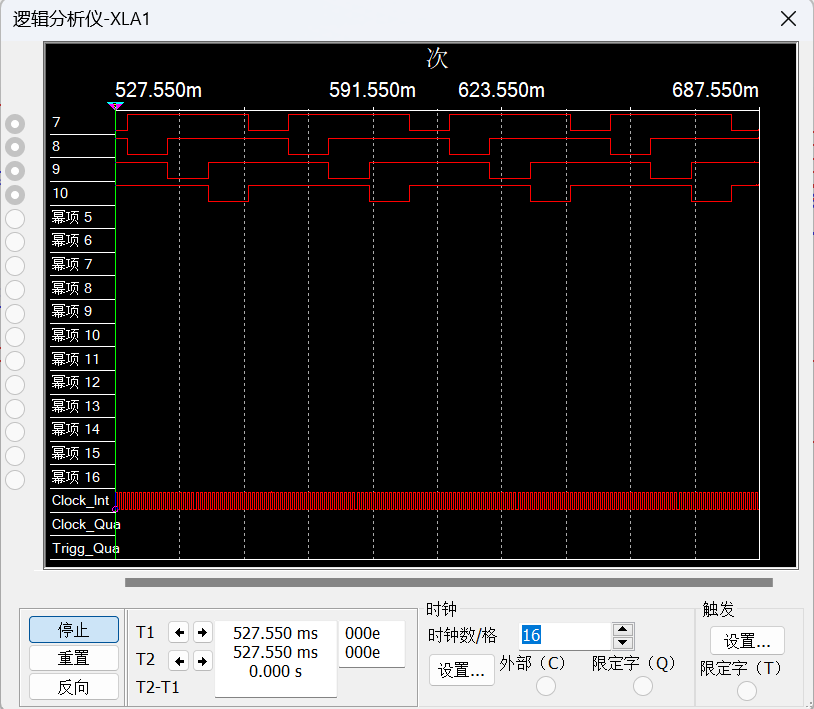
\includegraphics[width=0.6\textwidth]{逻辑分析仪.png}
    \caption{逻辑分析仪截图}
\end{figure}
上面四行是LED灯的输入电平,可以看到,低电平在依次循环右移,实现了流水灯功能。据此搭建的电路实物图如下所示
\begin{figure}[H]
    \centering
    \includegraphics[width=0.6\textwidth]{实物图 (2).jpg}
    \caption{电路实物图}
\end{figure}
上电测试,电路工作正常
\begin{figure}[H]
    \centering
    \begin{minipage}{0.4\textwidth}
    \centering
           \includegraphics[width=0.8\textwidth]{实物图 (1).jpg}
           
    \label{}
    \end{minipage}
    \hspace{0.05\textwidth}
    \begin{minipage}{0.4\textwidth}
    \centering
           \includegraphics[width=0.8\textwidth]{实物图 (3).jpg}
           
    \label{7474}
    \end{minipage}
\end{figure}
\begin{figure}[H]
    \centering
    \begin{minipage}{0.4\textwidth}
    \centering
           \includegraphics[width=0.8\textwidth]{实物图 (4).jpg}
           
    \label{}
    \end{minipage}
    \hspace{0.05\textwidth}
    \begin{minipage}{0.4\textwidth}
    \centering
           \includegraphics[width=0.8\textwidth]{实物图 (5).jpg}
           
    \label{7474}
    \end{minipage}
\end{figure}
\section{反思与总结}
本次实验是第一个时序逻辑电路实验。题目较为简单,但仍有一些值得关注的点
\begin{enumerate}
    \item 在最开始构思时,曾经想过用CLK信号编码,但是一来这种操作不常见,二来不符合题目使用两个D触发器的要求,并且,因为一片7474里面集成两个触发器,所以并不会节省芯片。所以这种操作并没有什么优点,遂放弃。
    \item 最开始在Multisim仿真中一直没有出现正确的现象,表现为逻辑分析仪波形正常,但是LED灯不亮,最后发现是脉冲源的高电平不够高,无法驱动LED灯。这种低级错误可能是由于实际搭建电路从来没有考虑过类似问题。
    \item 本问题只涉及到4种编码,但是在实际走线的时候出现了比较混乱的局面,一直出现不正确的流水现象,比如相邻的两个灯状态相同或者一个灯一直点亮或熄灭。最后的解决办法是,将实物电路图拍照,在图上标好代表的变量值,安排好走线。这种方法在以后处理更大规模的电路时可能比直接处理实物电路更加高效。
\end{enumerate}
\end{document}